\documentclass{article}

\usepackage{arxiv}
\usepackage[utf8]{inputenc} % allow utf-8 input
\usepackage[T1]{fontenc}    % use 8-bit T1 fonts
\usepackage{hyperref}       % hyperlinks
\usepackage{url}            % simple URL typesetting
\usepackage{booktabs}       % professional-quality tables
\usepackage{amsfonts}       % blackboard math symbols
\usepackage{nicefrac}       % compact symbols for 1/2, etc.
\usepackage{microtype}      % microtypography
\usepackage{lipsum}
\usepackage{graphicx,wrapfig}
\usepackage{caption}
\usepackage{booktabs}
\usepackage{subfig}
\usepackage{float}
\raggedbottom

\title{Diabetic Retinopathy Detection}

\author{
  David Unger\\
  3522491 \\
  M. Eng. Autonome Systeme\\
  University of Stuttgart\\
  \texttt{st172353@stud.uni-stuttgart.de} \\
  \And
  Nick Wagner\\
  3524444 \\
  B. Eng. Autonome Systeme\\
  University of Stuttgart\\
  \texttt{st175644@stud.uni-stuttgart.de} \\
}

% used for confusion matrix
\usepackage{babel}
\usepackage[table]{xcolor}
\usepackage{collcell}
\usepackage{hhline}
\usepackage{pgf}
\usepackage{multirow}
\def\colorModel{hsb} %You can use rgb or hsb
\newcommand\ColCell[1]{
  \pgfmathparse{#1<50?1:0}  %Threshold for changing the font color into the cells
    \ifnum\pgfmathresult=0\relax\color{white}\fi
  \pgfmathsetmacro\compA{0}      %Component R or H
  \pgfmathsetmacro\compB{#1/100} %Component G or S
  \pgfmathsetmacro\compC{1}      %Component B or B
  \edef\x{\noexpand\centering\noexpand\cellcolor[\colorModel]{\compA,\compB,\compC}}\x #1
  } 
\newcolumntype{E}{>{\collectcell\ColCell}m{0.4cm}<{\endcollectcell}}  %Cell width
\newcommand*\rot{\rotatebox{90}}
% end for confusion matrix

\begin{document}
\maketitle

\begin{abstract}
Diabetic retinopathy is an eye disease that can affect people suffering diabetes. It causes damage to the blood vessels of 
the eyes, deteriorates the eyesight and can lead in the worst case to blindness of the patient. It is important to 
detect the disease in an early stage to mitigate it as good as possible with an early treatment. Analyzing images of 
eyes and classify the severity of diabetic retinopathy is a challenging task that requires expert knowledge. To assist 
doctors and medical personnel, a classification model shall be trained to classify the severity automatically. 
\end{abstract}

% 1 %%%%%%%%%%%%%%%%%%%%%%%%%%%%%%%%%%%%%%%%%%%%%%%%%%%%%%%%%%%%%%%%%%%%%%%%%%%%%%%%%%%%%%%%%%%%%%%%%%%%%%%%%%%%%%%%%%%%%%
\section{Introduction}
Diabetic retinopathy is a complication of diabetes, which can cause damage the retina of the eye. 
If not detected early, this damage may cause cause vision impairment or even blindness. 
To treat this condition successfully, it has to be detected at an early stage, which is difficult due to minimal to no early warning signs. 
Furthermore, the different grades can only be distinguished by a trained professional due to its subtle symptoms.
Examples are leaking blood vessels, fatty deposits or retinal swelling.
Since this task is difficult even for trained professionals, an algorithm for automatic detection of the diabetic retinopathy grade is necessary.
This is the goal of this paper. 

The used dataset is the Indian Diabetic Retinopathy Image Dataset (IDRID), which is publicly available. It contains five class labels, which refer to 
the different eye disease grades (0-4).

% 2 %%%%%%%%%%%%%%%%%%%%%%%%%%%%%%%%%%%%%%%%%%%%%%%%%%%%%%%%%%%%%%%%%%%%%%%%%%%%%%%%%%%%%%%%%%%%%%%%%%%%%%%%%%%%%%%%%%%%%%
\section{Object Classification}
\subsection{Problem analysis}

To tackle the problem of diabetic retinopathy detection, several methods are possible. Because the dataset consists of 
ordinally scaled data of 5 classes, regression could be used to estimate the serverity of a case. In addition, a the problem 
can be handled as a classification problem after one-hot-encoding the labels. As a third option, one can define a threshold 
to define problematic diabetic retinopathy and non-problematic diabetic retinopathy and can handle the problem as a binary 
classification. Further, only binary and multiclass classification are anaylzed.

A binary classification has the advantage of higher accuracy, but lacks details, because the network only outputs 0 or 1
and no information about the exact serverity of the disease. Metrics are also easy to implement, because precision, 
recall and f1-score are standard implementations and nicely interpretable.

A multiclass classification has typically a lower accuracy, because the network needs to pick the right class among 
several classes. It provides the benefit or receiving richer information, i.e. the exact serverity of the disease.
Evaluating a multiclass classification problem becomes harder, because missclassifications can vary in their error.
Classifiying a class 1 as class 2 is for example less problematic than classifying class 1 as class 5.


\subsection{Architecture}
\begin{figure}[h]
  \centering
  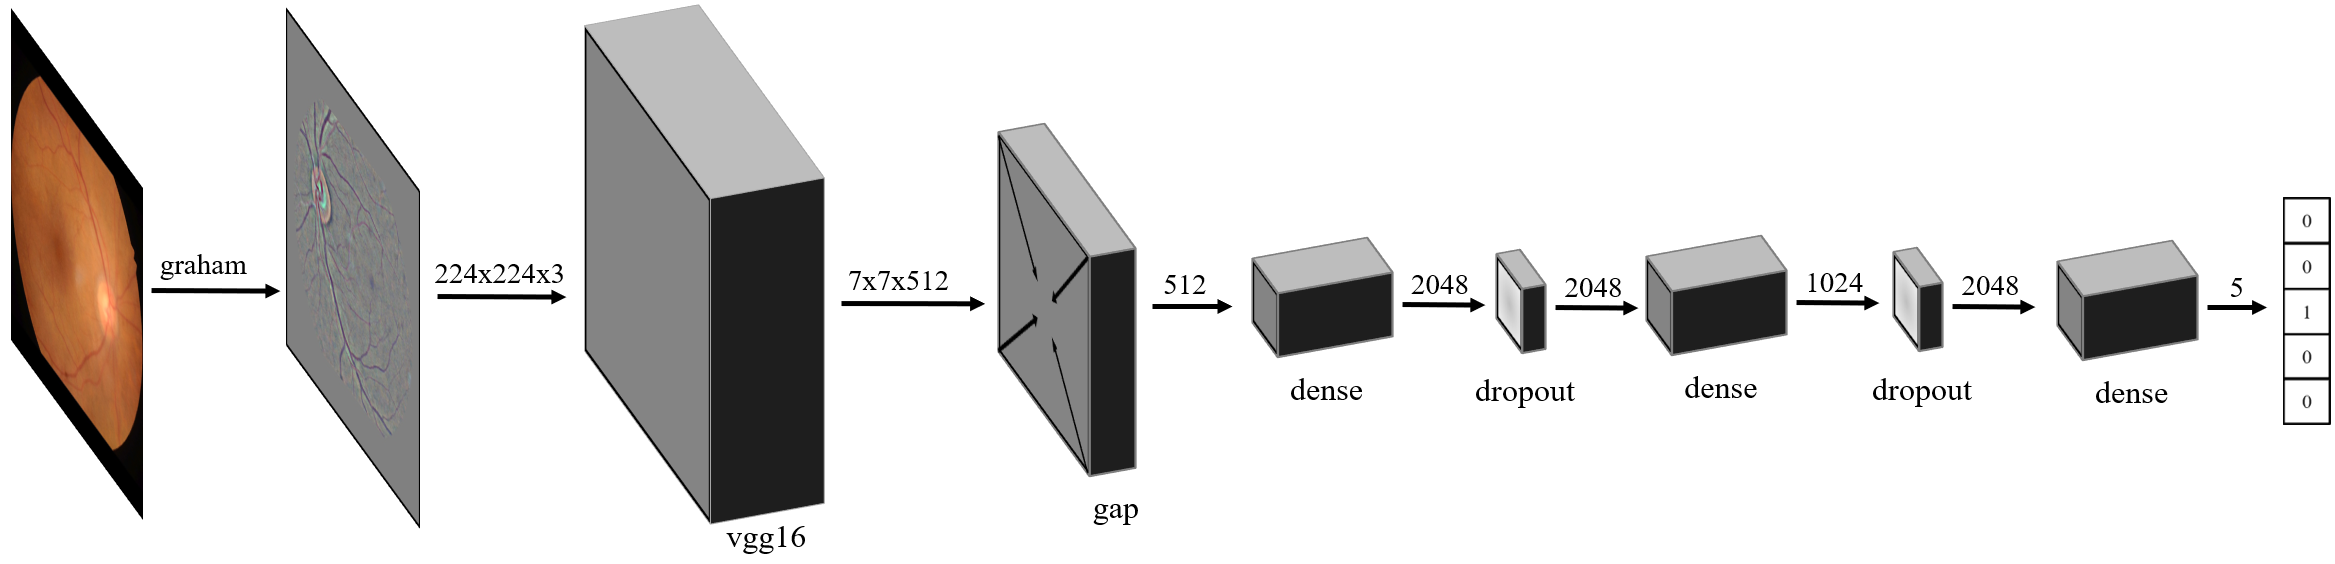
\includegraphics[width=1\textwidth]{2_2_architecture.png}\label{fig:architecture}
  \caption{Model architecture}
\end{figure}
The center piece of the architecture is a vgg16 transfer model that is trained on imagenet data. 
It's responsibility is to learn local features before the feature maps get average pooled.
Then three dense layers including dropout for regularization are used. The final output consists of five values that correspond
to the five diabetic retinopathy grade predictions.
The decision for this architecture is based on parameter optimization of many factors which get discussed in chapter \ref{ch_hyperparam}.
>> draw 3D architecture in powerpoint

To tackle the classification problem, we analyzed several model architectures that are composed of three parts: the 
base model, the conversion layer and the head of our model. For the base model we used ResNet50 and VGG16 with 
weights pretrained on ImageNet. We tried out the results with a fully trainable, partly trainable and not trainable
base model. As conversion layer we tested both, a flatten layer and global average pooling (GAP).
For the head we tried up to three hidden dense layers with different number of neurons per layer.

\subsection{Weight initialization}
Weight initialization refers to the initial values of parameters that are used in specific neural network layers.
Changing the initialization of the layers changes the starting point for the optimization process and potentially also the performance.
Keras initializes the weights of dense layers with the Glorot uniform initializer, which draws samples from a truncated uniform distribution.
Generally the goal is to avoid vanishing and exploding gradients, even better is if the variance of layer outputs is approximately one. [paper KUMAR]
Specifically for the ReLU activation function, this is achieved with the He initialization, which draws from a normal distribution with the following parameters. [paper HE]\\
\begin{minipage}{.5\linewidth}
  \begin{equation}
    \mu = 0
  \end{equation}
\end{minipage}
\begin{minipage}{.5\linewidth}
  \begin{equation}
    \sigma^2 = 2/N
  \end{equation}
\end{minipage}

This led to a faster training and performance increase of X percent.

\subsection{Augmentation}
Within the input pipeline three main types of augmentation are applied.
The goal is to make feature extraction easier for the network and increase the amount of input images which reduces overfitting.
\begin{itemize}
  \item[-] \textbf{Graham preprocessing:  [report kaggle]} \begin{itemize}
    \item[1.] rescale the eye radius to 300 pixels 
    \item[2.] subtract the local average color such that the local average gets mapped to gray
    \item[3.] clip the image to remove boundary effects
    \begin{figure}[h]
      \centering
      \subfloat[Original image]{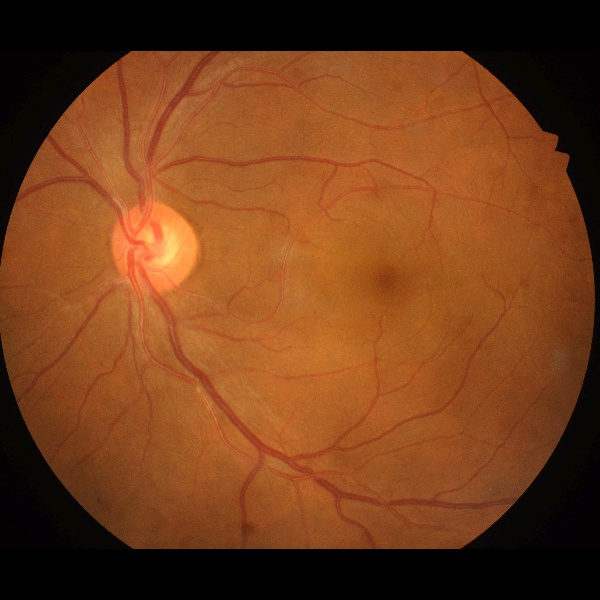
\includegraphics[width=0.15\textwidth]{IDRiD_060.jpg}\label{fig:IDRiD_backprop_orig}}
      \hspace{0.5cm}
      \subfloat[Processed image]{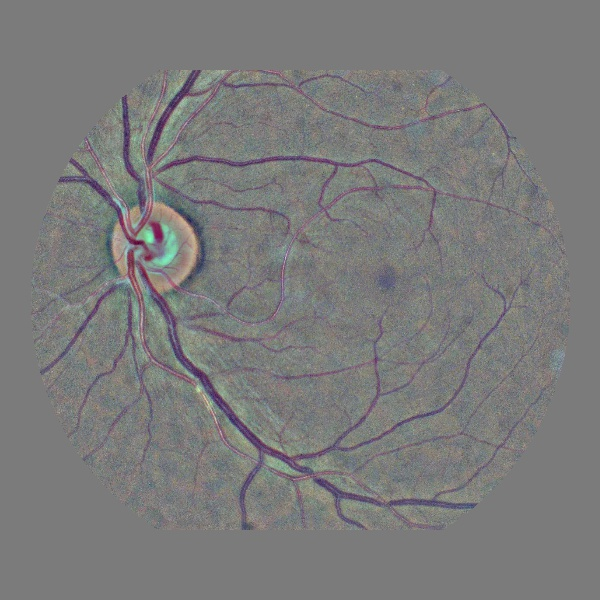
\includegraphics[width=0.15\textwidth]{IDRiD_060_graham.jpg}\label{fig:IDRiD_backprop_enh}}
      \caption{Graham pre-processing}
    \end{figure}] 
  %   \begin{figure}[h]
  %     \begin{minipage}[b]{.5\textwidth}
  %         \begin{center}
  %         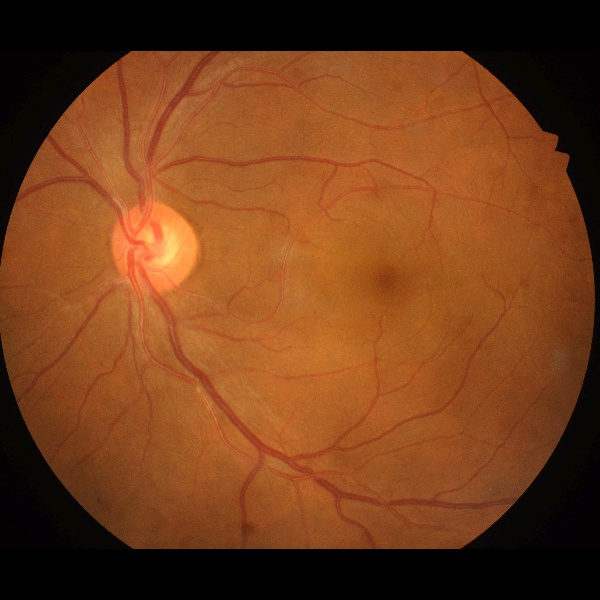
\includegraphics[width=.5\linewidth]{IDRiD_060.jpg}
  %         \captionsetup{justification=centering}
  %         \captionof{figure}{Original image}
  %         \label{fig:IDRiD}
  %         \end{center}
  %     \end{minipage}%
  %     \begin{minipage}[b]{.5\textwidth}
  %         \begin{center}
  %         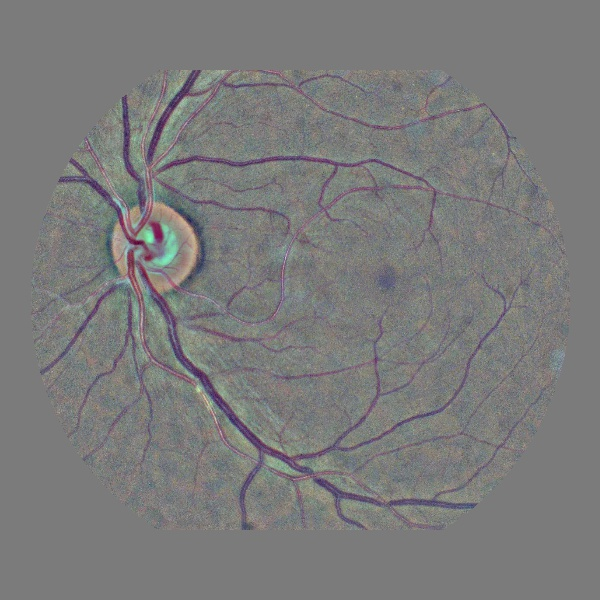
\includegraphics[width=.5\linewidth]{IDRiD_060_graham.jpg}
  %         \captionsetup{justification=centering}
  %         \captionof{figure}{Graham preprocessed image}
  %         \label{fig:IDRiD_graham}
  %         \end{center}
  %     \end{minipage}
  % \end{figure} 
  \end{itemize}   
  \item[-] \textbf{Color jittering:} Slight random changes to brightness, hue, saturation or contrast.
  \item[-] \textbf{Random cropping:} Crop a window that is slightly smaller than the image. Then resize to original size again.
\end{itemize}

% Dataset Balancing
\subsection{Dataset Balancing}
Taking a closer look at the sample distribution within the dataset \ref{tab:table1}, it is obviously imbalanced. This will inevitably lead to a trained model
that is fitted better to the overrepresented classes.

\renewcommand{\arraystretch}{1.2}
\begin{table}[h]
  \centering
  \begin{tabular}{|l|l|l|l|l|l|}
  \hline
  Label:   & 0   & 1  & 2   & 3  & 4  \\ \hline \hline
  \# train & 134 & 20 & 136 & 74 & 49 \\ \hline
  \# test  & 34  & 5  & 32  & 19 & 13 \\ \hline
  \end{tabular}
  \caption{Dataset sample distribution}
  \label{tab:table1}
  \end{table}

To avoid this, a method called oversampling is applied. Oversampling allows drawing underrepresented classes from the training set more often, 
such that all classes are equally represented when training the model.

\subsection{Training}
For training our model, we used categorical cross-entropy as loss function and experimented with the optimizer and 
learning rate. As optimizer we selected SGD with a momentum of 0.9 and Adam which both performed quite similar.

As learning rate, we tried 0.1, 0.01 and 0.001 from which latter performed best and further learning rate decay
showed no further improvement.

\subsection{Metrics}
Training deep neural networks requires some performance metrics indicating the success or failure of the model fitting. Accuracy
is easy to understand and to implement, but not suited for imbalanced data, because it doesn't take into account how well each 
single class is predicted. 
To overcome this, precision (how accurate was the model with its prediction) and recall (how thorough is a model with its prediction) can be used. 
Especially a combination of both, the f1-score is a metrics that indicates how well a classifier handles different classes.

For the diabetic retinopathy dataset, the f1-score comes with a drawback. The dataset is ordinally scaled, which means predicting 
a wrong class is not equally bad. As an example is predicting class 4 for the true class 0 much worse that predicting a 1. The
f1-score would count both missclassifications equally, while the Quadratic Weighted Kappa (QWC) metric takes the distance of 
the classification error into account.
% 3 %%%%%%%%%%%%%%%%%%%%%%%%%%%%%%%%%%%%%%%%%%%%%%%%%%%%%%%%%%%%%%%%%%%%%%%%%%%%%%%%%%%%%%%%%%%%%%%%%%%%%%%%%%%%%%%%%%%%%%
\section{Experiments}
\subsection{Procedure}
The training of the deep neural network classifier requires the selection of suitable hyperparameters that differ from
problem to problem. A useful strategy to find a good set of hyperparameters are parameter sweeps. Weights\&Biases is a 
python library that enables the easy implementation of sweeps. 

Hyperparameter optimization requires besides training and test dataset a third, the validation dataset, to evaluate the
model after hyperparameter tuning and to avoid overfitting on the hyperparameters. Because the given dataset only contains 
training and test data, the original training dataset was split into 80\% training data and 20\% validation data.

To perform many parameter sweeps, we stored out dataset in the cloud and used Google Colab as training server. 

\subsection{Hyperparameter selection}\label{ch_hyperparam}
As metrics for hyperparameter selection, we mainly used correlation with the validation-f1-score and 
compared the minimum, median and maximum run of each sweeped hyperparameter value with each other. 
Once most important hyperparameter is determined and selected, one needs to ensure that the second most important
parameter is not selected because of strong correlation with the most important one. Therefore, the independence can be 
guaranteed by filtering the sweep and selecting just runs with the best parameter one or by performing a new parameter sweep
with a fixed parameter one.

With this procedure, we selected the most important parameters as in table...:



\renewcommand{\arraystretch}{1.2}
\begin{table}[h]
  \centering
  \begin{tabular}{|l|l|}
  \hline
  Hyperparameter & Selected\\ \hline \hline
  Use Graham preprecessing & False \\ \hline
  Model architecture & ResNet50 \\ \hline
  Learning rate & 0.001 \\ \hline
  Balancing & true \\ \hline
  Flatten or GAP & GAP \\ \hline
  Number of dense neurons in layer N-3 & 4096 \\ \hline
  Number of dense neurons in layer N-1 & 0 \\ \hline
  \end{tabular}
  \caption{Dataset sample distribution}
  \label{tab:table2}
  \end{table}


\begin{figure}[h]
  \centering
  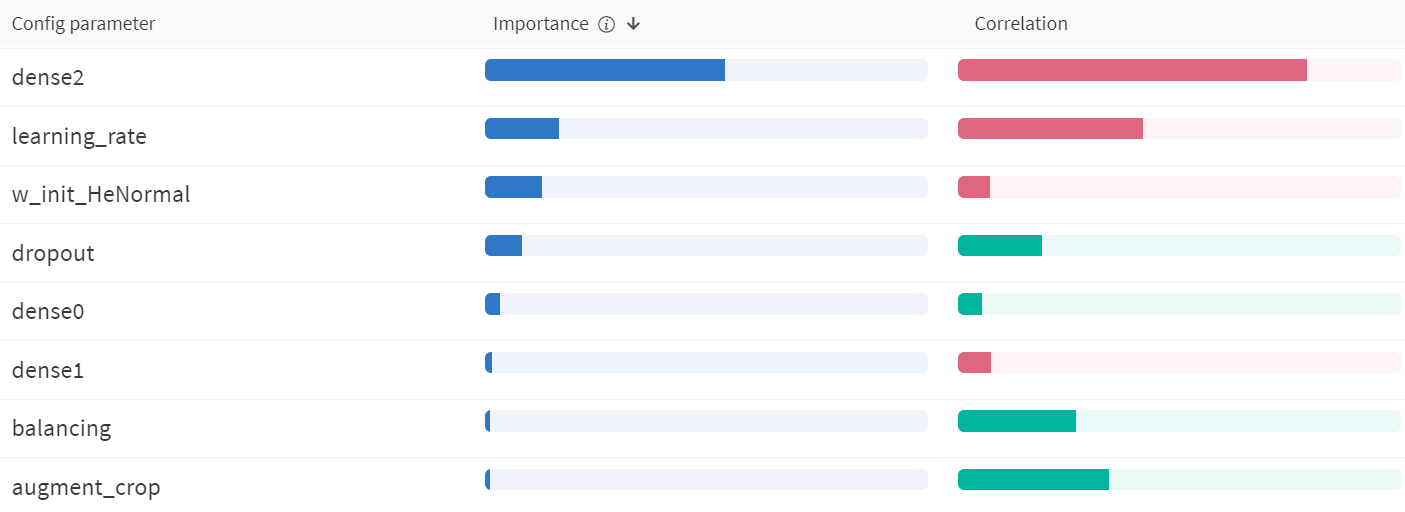
\includegraphics[width=0.8\textwidth]{3_2_parameter_importance.png}\label{fig:param_importance}
  \caption{Most important parameters with a sweep of 80 experiments}
\end{figure}

The following parameters show a big effect on the performance of the neural network on the validation data, 
why they are selected for the final classifier.

Balancing
...
% Deep Visualization
\subsection{Deep Visualization}
\subsubsection{Guided Backpropagation}
Guided Backpropagation belongs to the family of pixel-space gradient visualizations. 
The goal is to exploit the idea that neurons act like detectors of image features by using backpropagation.
What makes this backpropagation guided is that negative gradient are set to zero. This way, only pixels that are positively important to 
the output get highlighted. This method is not class-discriminative.  
\begin{figure}[h]
  \centering
  \subfloat[Original result]{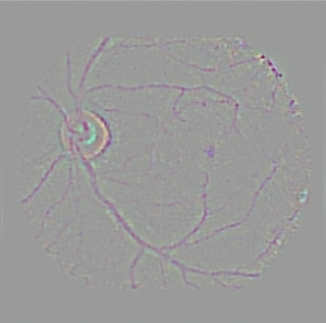
\includegraphics[width=0.15\textwidth]{IDRiD_060_backprop_orig.png}\label{fig:IDRiD_backprop_orig}}
  \hspace{0.5cm}
  \subfloat[Enhanced result]{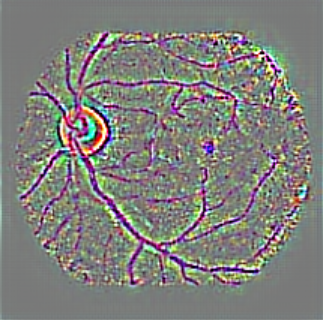
\includegraphics[width=0.15\textwidth]{IDRiD_060_backprop_enh.png}\label{fig:IDRiD_backprop_enh}}
  \caption{Guided Backpropagation}
\end{figure}
\subsubsection{CAM}
Class Activation Map (CAM) is class-discriminative and highlights relevant image regions, but in a less fine-grained manner
To achieve this, global average pooling has to be performed on the last feature maps of the last convolutional layer, followed by a dense layer as output.
The weights of this dense layer are then projected back to the convolutional feature maps which results in the class activation mappings.
As a consequence, it is hard to generalize this approach due to the architecture restrictions.
\subsubsection{GradCAM}
GradCAM is class-discriminative as well, but can be used by any CNN-based network without architectural adaptions.
Similar to CAM, it describes the activation as a linear combination of weighted feature maps. But in this case, the weights are calculated
by deriving the logit per class by the feature maps of the chosen convolutional layer. These gradients then get global average pooled, followed by a ReLU.
The ReLU leaves only feature with a positive impact behind, similar to how it is applied in Guided Backpropagation.
\subsubsection{Guided GradCAM}
Guided GradCAM combines the ideas of Guided Backpropagation with Class Activation Maps.
This makes GradCAM class-discriminative due to the localization of relevant image regions and high-resolution due pixel-space gradient visualization.
\begin{figure}[H]
  \centering
  \subfloat[Guided Backprop.]{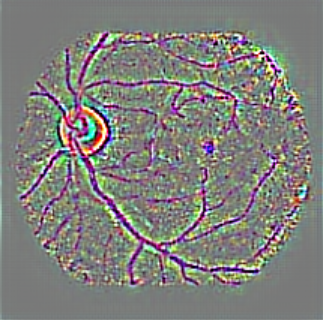
\includegraphics[width=0.15\textwidth]{IDRiD_060_backprop_enh.png}\label{fig:IDRiD_backprop_orig}}
  \hspace{0.5cm}
  \subfloat[gradCAM]{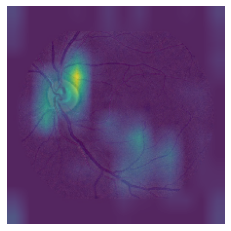
\includegraphics[width=0.15\textwidth]{IDRiD_060_gradCAM.png}\label{fig:IDRiD_backprop_enh}}
  \hspace{0.5cm}
  \subfloat[Guided gradCAM]{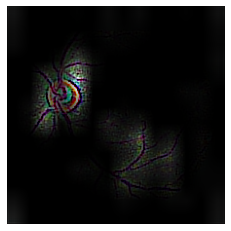
\includegraphics[width=0.15\textwidth]{IDRiD_060_guided_gradCAM.png}\label{fig:IDRiD_backprop_enh}}
  \caption{Guided Backpropagation}
  \small \textit{{Note: The chosen model architecture leads to graph issues within the gradCAM algorithm. The workaround affects the result negatively.
  A working example with another model and image can be found in the code within the "helper" folder.}}
\end{figure}

% 4 %%%%%%%%%%%%%%%%%%%%%%%%%%%%%%%%%%%%%%%%%%%%%%%%%%%%%%%%%%%%%%%%%%%%%%%%%%%%%%%%%%%%%%%%%%%%%%%%%%%%%%%%%%%%%%%%%%%%%%
\section{Results}
We trained and evaluated our algorithm on both, binary and multiclass classification.

For binary classification we performed a hyperparameter sweep and achieved without further optimization an f1-score of 0.87 on the 
validation data and of 0.82 on the test data.

% start confusion matrix
\newcommand\items{5}   %Number of classes
\arrayrulecolor{white} %Table line colors
\noindent\begin{tabular}{cc*{\items}{|E}|}
\multicolumn{1}{c}{} &\multicolumn{1}{c}{} &\multicolumn{\items}{c}{Predicted} \\ \hhline{~*\items{|-}|}
\multicolumn{1}{c}{} & 
\multicolumn{1}{c}{} & 
\multicolumn{1}{c}{\rot{Class 0}} & 
\multicolumn{1}{c}{\rot{Class 1}} & 
\multicolumn{1}{c}{\rot{Class 2}} & 
\multicolumn{1}{c}{\rot{Class 3}} & 
\multicolumn{1}{c}{\rot{Class 4}} \\ \hhline{~*\items{|-}|}
\multirow{\items}{*}{\rotatebox{90}{Actual}} 
&Class 0  & 29 &  2 &  2 &  0 &  1   \\ \hhline{~*\items{|-}|}
&Class 1  &  0 &  3 &  2 &  0 &  0   \\ \hhline{~*\items{|-}|}
&Class 2  &  7 &  1 & 15 &  3 &  6   \\ \hhline{~*\items{|-}|}
&Class 3  &  2 &  0 &  3 &  9 &  4   \\ \hhline{~*\items{|-}|}
&Class 4  &  4 &  0 &  1 &  1 &  7   \\ \hhline{~*\items{|-}|}
\end{tabular}
% end confusion matrix

For multiclass classification we optimized our model further and performed several sweep. Our finally selected model achieves 
a QWC score of 0.44 which would be rank 106 for the Kaggle challenge.
best binary + multiclass performance;
color coded confusion matrix


\bibliographystyle{unsrt}  
%\bibliography{references}  %%% Remove comment to use the external .bib file (using bibtex).
%%% and comment out the ``thebibliography'' section.


%%% Comment out this section when you \bibliography{references} is enabled.
\begin{thebibliography}{1}

\bibitem{kumar2017weight}
Siddharth Krishna Kumar.
\newblock On weight initialization in deep neural networks.
\newblock {\em arXiv:1704.08863}, 2017.

\bibitem{kumar2017weight}
name.
\newblock title.
\newblock In {\em Frontiers in Handwriting Recognition (ICFHR), 2014 14th
  International Conference on}, pages 417--422. IEEE, 2014.

Guided Backpropagation: https://arxiv.org/abs/1412.6806

\end{thebibliography}

\end{document}
